\chapter{\babDua}
Membuat desain sebuah perangkat ic membutuhkan proses yang panjang dan sumberdaya manusia yang banyak, serta tingkat ketelitian yang tinggi. Oleh karenanya di butuhkan biaya yang tidak kecil dan waktu yang cukup lama hanya untuk membuat sebuah desain IC. Dengan kerumitan yang tinggi serta waktu yang lama dalam setiap prosesnya kadang pihak yang tak bertanggung jawab melakukan kecurangna dengan mecuri desain untuk memotong waktu dan biaya yang di butuhkan utuk produksi. sehingga menjadi masalah dalam dunia permanufakturan ic.

\section{Large Scale Integration}
Berdasarkan \cite{latex.intro}: \\ 
\begin{tabular}{| p{13cm} |}
	\hline 
	\\
	LaTeX is a family of programs designed to produce publication-quality typeset documents. It is particularly strong when working with mathematical symbols. \\	
	The history of LaTeX begins with a program called TEX. In 1978, a 
	computer scientist by the name of Donald Knuth grew frustrated with the mistakes that his publishers made in typesetting his work. He decided to create a typesetting program that everyone could easily use to typeset documents, particularly those that include formulae, and made it freely available. The result is TEX. \\	
	Knuth's product is an immensely powerful program, but one that does focus very much on small details. A mathematician and computer scientist by the name of Leslie Lamport wrote a variant of TEX called LaTeX that focuses on document structure rather than such details. \\
	\\
	\hline
\end{tabular}

\vspace*{0.8cm}

Dokumen \latex~sangat mudah, seperti halnya membuat dokumen teks biasa. Ada beberapa perintah yang diawali dengan tanda '\bslash'. 
Seperti perintah \bslash\bslash~yang digunakan untuk memberi baris baru. Perintah tersebut juga sama dengan perintah \bslash newline. 
Pada bagian ini akan sedikit dijelaskan cara manipulasi teks dan  perintah-perintah \latex~yang mungkin akan sering digunakan. Jika ingin belajar hal-hal dasar mengenai \latex, silahkan kunjungi:

\begin{itemize}
	\item \url{http://frodo.elon.edu/tutorial/tutorial/}, atau \item \url{http://www.maths.tcd.ie/~dwilkins/LaTeXPrimer/}
\end{itemize}

\section{Arus Pengembangan LSI}

Agar dapat menggunakan \latex~(pada konteks hanya sebagai pengguna), Anda tidak perlu banyak tahu mengenai hal-hal didalamnya. 
Seperti halnya pembuatan dokumen secara visual (contohnya Open Office (OO) Writer), Anda dapat menggunakan \latex~dengan cara yang sama. 
Orang-orang yang menggunakan \latex~relatif lebih teliti dan terstruktur mengenai cara penulisan yang dia gunakan, \latex~memaksa Anda untuk seperti itu.

Kembali pada bahasan utama, untuk mencoba \latex~Anda cukup mendownload kompiler dan IDE. Saya menyarankan menggunakan Texlive dan Texmaker. Texlive dapat didownload dari \url{http://www.tug.org/texlive/}. 
Sedangkan Texmaker dapat didownload dari 
\url{http://www.xm1math.net/texmaker/}. 
Untuk pertama kali, coba buka berkas thesis.tex dalam template yang Anda miliki pada Texmaker. Dokumen ini adalah dokumen utama. 
Tekan F6 (PDFLaTeX) dan Texmaker akan mengkompilasi berkas tersebut menjadi berkas PDF. Jika tidak bisa, pastikan Anda sudah menginstall Texlive. Buka berkas tersebut dengan menekan F7. Hasilnya adalah sebuah dokumen yang sama seperti dokumen yang Anda baca saat ini. 

\section{Kemungkinan Serangan Desain LSI}

Hal pertama yang mungkin ditanyakan adalah bagaimana membuat huruf tercetak tebal, miring, atau memiliki garis bawah. 
Pada Texmaker, Anda bisa melakukan hal ini seperti halnya saat mengubah dokumen dengan OO Writer. Namun jika tetap masih tertarik dengan cara lain, ini dia: 

\begin{itemize}
	\item \bo{Bold} \\
		Gunakan perintah \bslash textbf$\lbrace\rbrace$ atau 
		\bslash bo$\lbrace\rbrace$. 
	\item \f{Italic} \\
		Gunakan perintah \bslash textit$\lbrace\rbrace$ atau 
		\bslash f$\lbrace\rbrace$. 
	\item \underline{Underline} \\
		Gunakan perintah \bslash underline$\lbrace\rbrace$.
	\item $\overline{Overline}$ \\
		Gunakan perintah \bslash overline. 
	\item $^{superscript}$ \\
		Gunakan perintah \bslash $\lbrace\rbrace$. 
	\item $_{subscript}$ \\
		Gunakan perintah \bslash \_$\lbrace\rbrace$. 
\end{itemize}

Perintah \bslash f dan \bslash bo hanya dapat digunakan jika package 
uithesis digunakan. 

\section{Mengatasi Serangan terhadap Desain LSI}

Setiap gambar dapat diberikan caption dan diberikan label. Label dapat digunakan untuk menunjuk gambar tertentu.  Jika posisi gambar berubah, maka nomor gambar juga akan diubah secara otomatis. Begitu juga dengan seluruh referensi yang menunjuk pada gambar tersebut. Contoh sederhana adalah \pic~\ref{fig:testGambar}. Silahkan lihat code \latex~dengan nama bab2.tex untuk melihat kode lengkapnya. Harap diingat bahwa caption untuk gambar selalu terletak dibawah gambar.

\begin{figure}
	\centering
	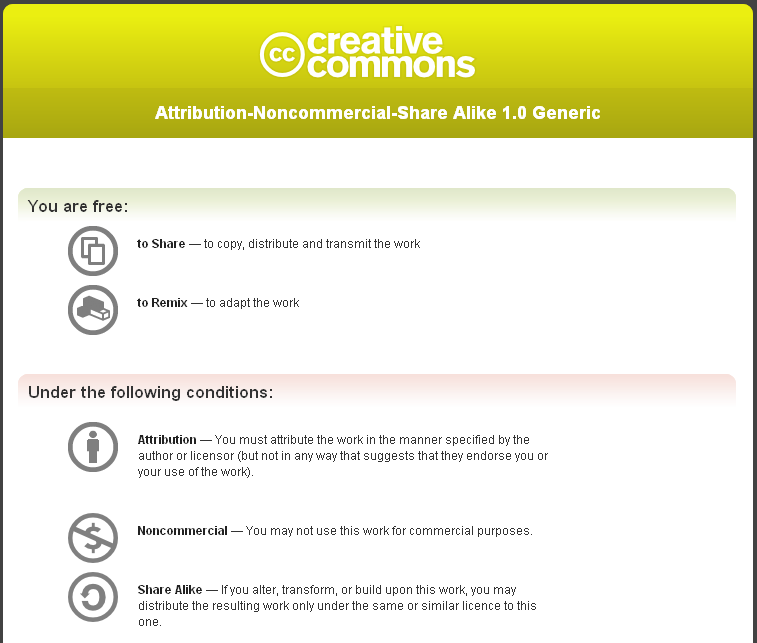
\includegraphics[width=0.50\textwidth]
		{pics/creative_common.png}
	\caption{\license.}
	\label{fig:testGambar}
\end{figure}

\section{Cara yang Diajukan Penulis}

Seperti pada gambar, tabel juga dapat diberi label dan caption.  Caption pada tabel terletak pada bagian atas tabel. Contoh tabel sederhana dapat dilihat pada \tab~\ref{tab:tab1}.

\begin{table}
	\centering
	\caption{Contoh Tabel}
	\label{tab:tab1}
	\begin{tabular}{| l | c r |}
		\hline
		& kol 1 & kol 2 \\ 
		\hline
		baris 1 & 1 & 2 \\
		baris 2 & 3 & 4 \\
		baris 3 & 5 & 6 \\
		jumlah  & 9 & 12 \\
		\hline
	\end{tabular}
\end{table}

Ada jenis tabel lain yang dapat dibuat dengan \latex~berikut 
beberapa diantaranya. Contoh-contoh ini bersumber dari 
\url{http://en.wikibooks.org/wiki/LaTeX/Tables}

\begin{table}
	\centering
	\caption{An Example of Rows Spanning Multiple Columns}
	\label{row.spanning}
	\begin{tabular}{|l|l|*{6}{c|}}
  		\hline % create horizontal line
  		No & Name & \multicolumn{3}{|c|}{Week 1} & \multicolumn{3}{|c|}{Week 2} \\
  		\cline{3-8} % create line from 3rd column till 8th column
  		& & A & B & C & A & B & C\\
  		\hline
  		1 & Lala & 1 & 2 & 3 & 4 & 5 & 6\\
  		2 & Lili & 1 & 2 & 3 & 4 & 5 & 6\\
  		3 & Lulu & 1 & 2 & 3 & 4 & 5 & 6\\
  		\hline
	\end{tabular}
\end{table}

\begin{table}
	\centering
	\caption{An Example of Columns Spanning Multiple Rows}
	\label{column.spanning}
	\begin{tabular}{|l|c|l|}
		\hline
		Percobaan & Iterasi & Waktu \\
		\hline
		Pertama & 1 & 0.1 sec \\ \hline
		\multirow{2}{*}{Kedua} & 1 & 0.1 sec \\
 		& 3 & 0.15 sec \\ 
 		\hline
		\multirow{3}{*}{Ketiga} & 1 & 0.09 sec \\
 		& 2 & 0.16 sec \\
 		& 3 & 0.21 sec \\ 
 		\hline
	\end{tabular}
\end{table}

\begin{table}
	\centering
	\caption{An Example of Spanning in Both Directions Simultaneously}
	\label{mix.spanning}
	\begin{tabular}{cc|c|c|c|c|}
		\cline{3-6}
		& & \multicolumn{4}{|c|}{Title} \\ \cline{3-6}
		& & A & B & C & D \\ \hline
		\multicolumn{1}{|c|}{\multirow{2}{*}{Type}} &
		\multicolumn{1}{|c|}{X} & 1 & 2 & 3 & 4\\ \cline{2-6}
		\multicolumn{1}{|c|}{}                        &
		\multicolumn{1}{|c|}{Y} & 0.5 & 1.0 & 1.5 & 2.0\\ \cline{1-6}
		\multicolumn{1}{|c|}{\multirow{2}{*}{Resource}} &
		\multicolumn{1}{|c|}{I} & 10 & 20 & 30 & 40\\ \cline{2-6}
		\multicolumn{1}{|c|}{}                        &
		\multicolumn{1}{|c|}{J} & 5 & 10 & 15 & 20\\ \cline{1-6}
	\end{tabular}
\end{table}